\section{Differentiable Spatial Routing and Physical Compression}
\label{sec:method}

\subsection{Architecture and actual sequence reduction}

For an image of size $H\times W$ and patch size $p$, let
$N=(H/p)(W/p)$ denote the number of patch slots, excluding a protected class
token. The main configuration uses $p=8$, width $d=384$, six attention heads,
six local blocks, and six latent blocks. At $224\times224$, the local encoder
processes $N+1=785$ tokens in every block. Its attention window is a
one-dimensional band extending 16 sequence positions in each direction,
with global attention for the class query. It is not a $16\times16$ spatial
window. Two-dimensional geometry enters through the routing support below.

The local encoder first computes all six layer outputs,
$H^{(1)},\ldots,H^{(L)}$. Routing then starts from the last output,
$X^{(0)}=H^{(L)}$, using a separate metric derived from each $H^{(\ell)}$.
Each routing step retains the complete slot tensor. Only after these steps
are completed does a hard gather physically reduce the sequence. This order
is essential: earlier local blocks do not benefit from progressively shorter
sequences. Figure~\ref{fig:architecture} depicts the executed dataflow.

\begin{figure}[t]
\centering
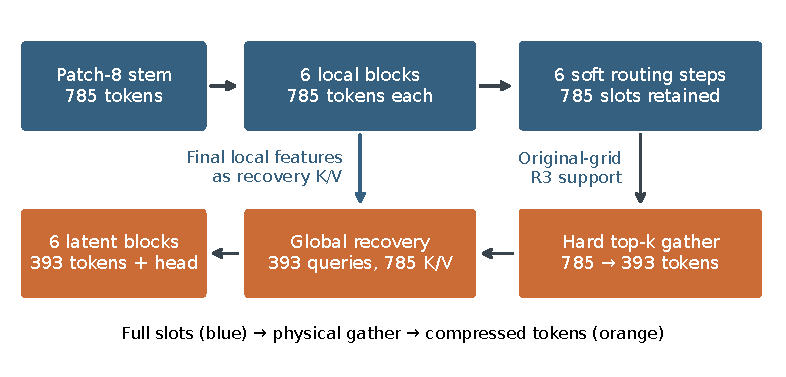
\includegraphics[width=\linewidth]{figures/architecture.pdf}
\caption{Main \mn{} dataflow at 224 pixels, rebuilt from the final
architecture on slide 3 of the collaborator deck and reconciled with the
executed classifier. All local blocks and soft-routing steps retain 785 slots.
The exact-budget gather is the first physical reduction; recovery then reads
the pre-transport final local features. Patch counts in the boxes exclude the
class token.}
\label{fig:architecture}
\end{figure}

\subsection{Original-grid eligibility}

Index patch slots by $i\in\{0,\ldots,N-1\}$ and define original coordinates
\begin{equation}
 u_i=\left(\left\lfloor i/(W/p)\right\rfloor,\ i\bmod(W/p)\right).
\end{equation}
At step $\ell$, patches are partitioned into donor and receiver sets
$A_\ell$ and $B_\ell$. Training uses a random partition for each sample;
evaluation alternates deterministic odd/even partitions across steps. The
class token belongs to neither merging set. For donor $i$, eligible receivers
are
\begin{equation}
 \mathcal E_i^{(\ell)}(R)=
 \{j\in B_\ell:\|u_i-u_j\|_2\leq R\}.
 \label{eq:support}
\end{equation}
Coordinates refer to the original slots throughout routing. They are not
replaced by the centers of the accumulated feature content. The main choice
is $R=3$ patch spacings. The global control removes this spatial constraint;
the flattened control uses the release's one-dimensional matching window
with width parameter 8.

Let $z_i^{(\ell)}$ be the normalized output of a learned $384\to64$ metric
projection applied to $H_i^{(\ell)}$. Its input gradient is scaled by 0.1
without changing its forward value. Following the inherited relaxed-routing
construction, eligible similarities define
\begin{align}
 s_{ij}&=\langle z_i^{(\ell)},z_j^{(\ell)}\rangle/\tau_1,\\
 e_i&=\sum_{j\in\mathcal E_i^{(\ell)}}\exp(s_{ij}),
 \qquad
 q_{ij}=\frac{\exp(s_{ij})}{e_i}
 \quad (j\in\mathcal E_i^{(\ell)}).
\end{align}
A threshold-based soft top-$k$ operator converts row energies $e_i$ into donor
weights $g_i$, with the step's scheduled merge budget $k_\ell$ as its target.
Writing $F$ for its smooth monotone threshold function, the construction has
the form
\begin{equation}
 g_i=F(\alpha\bar e_i-\theta),\qquad
 \sum_i g_i\approx k_\ell,
 \label{eq:softtopk}
\end{equation}
where the data-dependent threshold $\theta$ is solved in parallel after
sorting rather than by $k_\ell$ serial selections. This follows the
threshold-adjusted soft top-$k$ construction of Su~\cite{sujianlin2024topk}.
We use $\tau_1=1$ and multiplicative soft-selection scale $\alpha=30$. The
assignment is $a_{ij}=g_iq_{ij}$ on eligible edges and zero elsewhere, with
row-sum stabilization in the implementation. Empty rows have zero assignment.
If fewer eligible donor rows exist than the requested budget, the spatial
path raises an error instead of routing outside the support. Our notation
suppresses the implementation's numerical clamps and straight-through
stabilizers; it does not assume the relaxed weights are exact binary choices.

\subsection{Mass transfer and fixed-budget selection}

Each slot carries a nonnegative mass $m_i$, initialized to one. For a donor
$i$ and a receiver $j$, soft transport updates masses and receiver features as
\begin{align}
 m'_i &=m_i\left(1-\sum_j a_{ij}\right),\qquad X'_i=X_i,\\
 m'_j &=m_j+\sum_i a_{ij}m_i,\\
 X'_j &=\frac{m_jX_j+\sum_i a_{ij}m_iX_i}{m'_j}.
 \label{eq:transport}
\end{align}
The code clamps residual donor fractions and receiver denominators for
numerical stability. Donor slots remain in the tensor even when their mass
is small. Thus soft transport and token deletion are different operations.
The main spatial path evaluates a sparse neighbor list and uses indexed
transport; a dense score-then-mask path is available as a reference.

For compression parameter $\lambda$, the final number of patch carriers is
\begin{equation}
 K=N-\left\lfloor N\frac{\lambda-1}{\lambda}\right\rfloor.
 \label{eq:budget}
\end{equation}
The model gathers the $K$ largest-mass patches and prepends the protected
class token. At $\lambda=2$, $K=392$ at 224 pixels and $K=1152$ at 384 pixels.
At $\lambda=2$, the six soft donor-budget targets are
$(65,65,65,65,65,67)$ at 224 pixels and $(192,192,192,192,192,192)$ at 384.
The carrier count is fixed by configuration; the selected locations depend
on the input. A soft top-$K$ surrogate supplies straight-through gradients
through the selected features via $1+g-\operatorname{stopgrad}(g)$; it does
not differentiate every gather index. During training an auxiliary head contribution
is added to the main logits, with maximum weight 0.05; it is absent during
evaluation. This is a logit contribution, not a separately reported auxiliary
cross-entropy loss.

The default source-tracing mode maintains a detached mass-weighted center of
the flattened indices. It uses these values to sort selected carriers; it
does not retain the full source-membership matrix. Selected features $Q$
then undergo residual recovery,
\begin{equation}
 Y=Q+\operatorname{CrossAttn}(Q,H^{(L)},H^{(L)}).
 \label{eq:recovery}
\end{equation}
Recovery is global in this mode. Six global latent blocks process $K+1$
tokens, with no further merging. The class representation feeds the
classification head.

\subsection{Mass-aware attention and a fused implementation path}

Latent attention retains proportional attention by adding the logarithm of
selected carrier mass to each key logit. For per-head dimension $d_h$,
\begin{equation}
 \operatorname{Attn}(Q,K,V;m)=
 \operatorname{softmax}\!\left(\frac{QK^\top}{\sqrt {d_h}}
 +\mathbf 1\log(m)^\top\right)V.
 \label{eq:mass-attn}
\end{equation}
The bias is rank one across query positions. It can therefore be represented
without an explicit $K\times K$ bias matrix. Define
\begin{equation}
\widehat Q=[Q,\sqrt {d_h}\,\mathbf 1],\qquad
 \widehat K=[K,\log m].
\end{equation}
Calling standard scaled dot-product attention on $(\widehat Q,\widehat K,V)$
with scale $1/\sqrt {d_h}$ gives exactly the logits in
Equation~\eqref{eq:mass-attn}. The implementation pads the augmented head
dimension to a multiple of eight and passes the tensors to the unmodified
FlashAttention kernel~\cite{flashattn2022}; it does not materialize a dense
bias matrix.

\subsection{What the geometry and complexity claims mean}

Equation~\eqref{eq:support} bounds a single transport edge. It does not bound
the spatial extent of all original constituents after multiple steps: a
sequence of locally permitted transfers can travel farther. Moreover,
$H^{(L)}$ already contains contextual information and
Equation~\eqref{eq:recovery} reads globally. The constraint therefore concerns
routing support, not the entire model's receptive field or semantic
segmentation boundaries.

The distinction between slots and carriers also determines cost. Local
attention projections and MLPs still process $N+1$ tokens per layer.
Recovery has attention terms proportional to $NKd$, and latent self-attention
has terms proportional to $K^2d$. For fixed $\lambda$, both retain quadratic
terms in $N$. Sparse routing avoids a dense donor--receiver assignment during
the forward pass, but initialization still constructs an $N\times N$
Boolean adjacency buffer. Neither a linear-memory claim for the complete
implementation nor an end-to-end speedup follows from the sparse scorer alone.

\subsection{Measured routing structure: reserved visualization}
\label{sec:pending-routing}
\pendingslot{P06}{Trace actual routing on trained ImageNet examples}{The
figure is reserved for measured outputs, not an architectural illustration.}

Preselect validation image IDs and include typical and unsuccessful cases.
For each layer export the donor/receiver partition, eligible edges, transport
weights, selected carriers and token masses. To visualize original-source
membership, enable a verified membership trace: the default flattened-index
center cannot reconstruct it. Report the sampling rule and checkpoint
identity. Local edges alone do not establish semantic-boundary preservation;
that claim requires an annotation source and an explicit metric.

\begin{figure}[htbp]\centering
\pendingfigure{P06: images, routing edges, carriers, and a failure case}{3.8cm}
\caption{Reserved trained-checkpoint routing visualization [P06]. No
synthetic image or hand-drawn assignment is used as a model observation.}
\label{fig:pending-routing}\end{figure}
\pendingtext

